\documentclass{article}
\usepackage[utf8]{inputenc}
\usepackage{graphicx}
\usepackage{tikz}
\usepackage{float}
\usetikzlibrary{positioning,fit,calc,arrows.meta, shapes}
\graphicspath{ {images/} }

%Tot això hauria d'anar en un pkg, però no sé com és fa
\newcommand*{\assignatura}[1]{\gdef\1assignatura{#1}}
\newcommand*{\grup}[1]{\gdef\3grup{#1}}
\newcommand*{\professorat}[1]{\gdef\4professorat{#1}}
\renewcommand{\title}[1]{\gdef\5title{#1}}
\renewcommand{\author}[1]{\gdef\6author{#1}}
\renewcommand{\date}[1]{\gdef\7date{#1}}
\renewcommand{\maketitle}{ %fa el maketitle de nou
    \begin{titlepage}
        \raggedright{UNIVERSITAT DE LLEIDA \\
            Escola Politècnica Superior \\
            Grau en Enginyeria Informàtica\\
            \1assignatura\\}
            \vspace{5cm}
            \centering\huge{\5title \\}
            \vspace{3cm}
            \large{\6author} \\
            \normalsize{\3grup}
            \vfill
            Professorat : \4professorat \\
            Data : \7date
\end{titlepage}}
%Emplenar a partir d'aquí per a fer el títol : no se com es fa el package
%S'han de renombrar totes, inclús date, si un camp es deixa en blanc no apareix

\tikzset{
	%Style of nodes. Si poses aquí un estil es pot reutilitzar més facilment
	pag/.style = {circle, draw=black,
                           minimum width=0.75cm, font=\ttfamily,
                           text centered}
}
\renewcommand{\figurename}{Figura}
\title{Primera pràctica d'Inteligència Artificial}
\author{Joaquim Picó Mora}
\date{Divendres 15 de Novembre}
\assignatura{Inteligència Artificial}
\professorat{Carlos Ansotegui}
\grup{PraLab1}

%Comença el document
\begin{document}
\maketitle
\thispagestyle{empty}

\newpage
\pagenumbering{roman}
\tableofcontents
\newpage
\pagenumbering{arabic}

\section{Taula Evaluació Experimental}
\begin{figure}[h!]
	\centering
	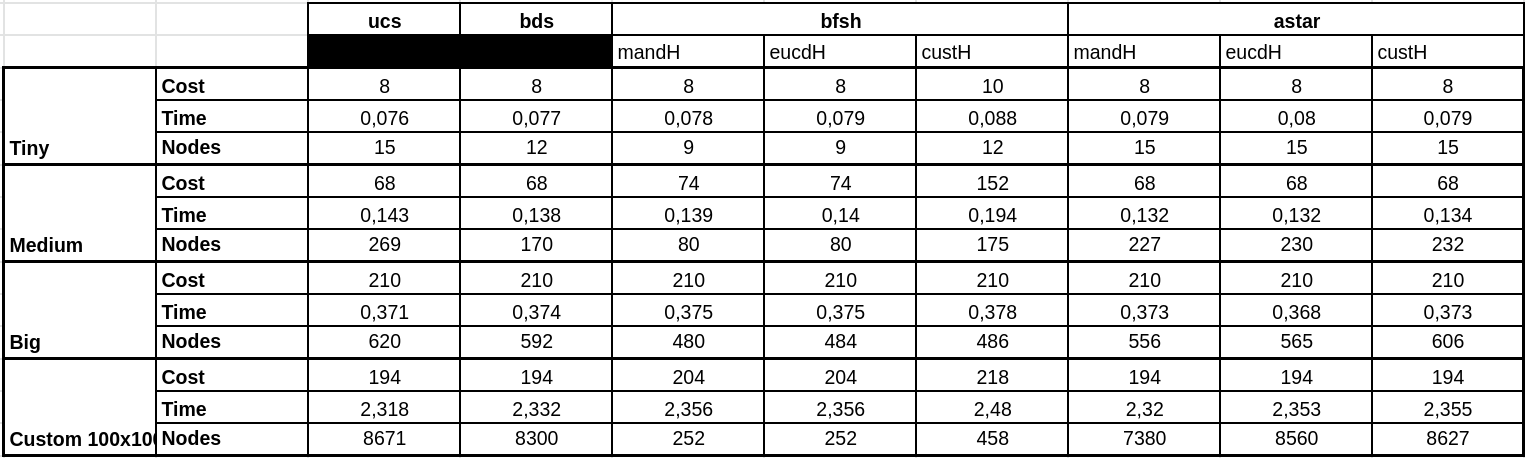
\includegraphics[width=0.7\textheight]{taula.png}
	\caption{Taula Evaluació Experimental.}
	\label{tee}
\end{figure}
\section{Algoritmes}
%
\subsection{Uniform Cost Search}
L'ucs és caracteritza per expandir sempre el node al que s'ha arribat amb el menor cost. Per a realitzar aixó he declarat la frontera com una cua per prioritat, fent així que cada cop que es tregui un element d'ella per a expandir-lo sigui el que te el cost més baix ja que la llista és trovarà ordenada per prioritat. 
\\\\
La principal característica d'aquest algorísme i que el fa diferir del Breath First Search és que si trobem un node n1 a la frontera que té un cost determinat, i un altre node n2 el qual ens porta al mateix estat que n1 i amb menor cost. Aleshores afegirem aquest segón node  a la frontera, i la mateixa cua per prioritat fara que n2 s'expandeixí abans que n1 ja que tindrà un cost menor i per tant una major prioritat.
\\\\
Aquest algoritme ens trobarà sempre el camí optim a la solució. En aquest cas però, al ser el cost lineal, l'espai d'estats finit, el factor de ramificació també finit i havent-hi solució, ens trobarà el camí optim, però executanse de forma identica a l'algoritme Breath First Search
\\\\
Podem veure en la Figura1 que l'ucs de tots els algoritmes proposats és el menys eficient en quant a espai. En canvis, el temps d'execució és molt proper al de tots els altres algorismes.

\end{document}